\documentclass{beamer}
 
\usepackage[czech]{babel}
\usepackage[utf8]{inputenc}
\usepackage{graphicx}
\graphicspath{ {img/} } 
 
%Titulní stránka
\usecolortheme{crane}
\title{Bitcoin}
\author{Jan Koscielniak}
\institute{VUT FIT}
\date{2016}
 
 
 
\begin{document}
 
\frame{\titlepage}
 
\begin{frame}
\frametitle{Co je to bitcoin?}
\begin{figure}[h]

\includegraphics[height=2.5cm]{bitcoinlogo}
\centering
\end{figure}
\begin{itemize}
\item Bitcoin je decentralizovaná elektronická kryptoměna
\item Vytvořil ji v~roce 2008 Satoshi Nakamoto
\item Od roku 2009 je open source
\item Je Peer-2-Peer \,--\, přímá komunikace mezi uživateli
\end{itemize}
\end{frame}

\begin{frame}
\frametitle{Jak Bitcoin funguje?}
\begin{itemize}
\item Síť je tvořena \emph{bloky}, které slouží k~potvrzování transakcí a uvolňování nových bitcoinů do oběhu
\item Ty lze \uv{těžit} pomocí speciálního software, který počítá složité matematické úlohy
\item Po vyřešení problému se blok zpropaguje do globání sítě - blockchainu
\end{itemize}
\end{frame} 

\begin{frame}
\frametitle{Jaké jsou výhody Bitcoinu?}
\begin{itemize}
\item V~blockchainu je zaznamenána každá transakce od začátku fungování sítě
\item Transakce nelze podvrhnout
\item Měnu nelze kontrolovat ani řídit
\end{itemize}
\end{frame}

\begin{frame}
\frametitle{Hodnota bitcoinu}
\begin{itemize}
\item Hodnota bitcoinu je velmi volatilní \,--\, ve špičce dosahovala více než 11 000 USD (konec roku 2013)
\end{itemize}
\begin{figure}[h]
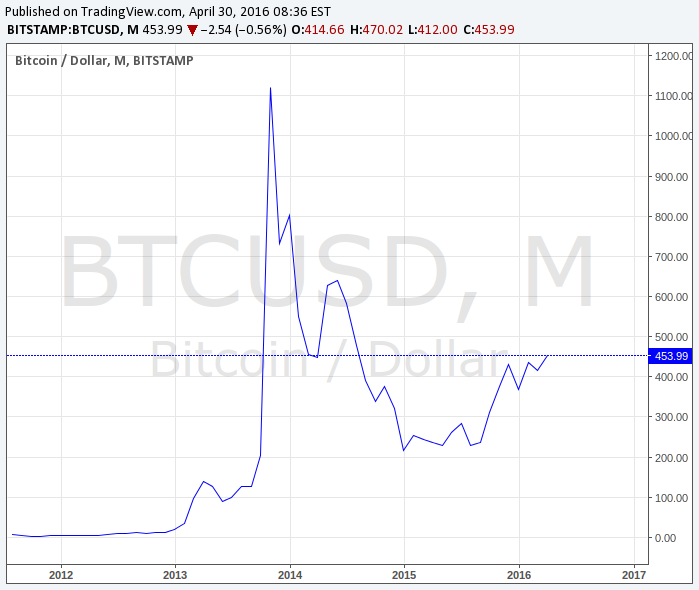
\includegraphics[height=5cm]{kurz}
\centering
\end{figure}
\end{frame}

\begin{frame}
\frametitle{Výhody bitcoinu}
\begin{itemize}
\item Absolutní kontrola nad vlastními bitcoiny \,--\, žádné zpoplatněné \uv{účty}
\item Velmi nízké, nebo žádné poplatky za transakce (lze zaplatit za prioritní potvrzení do blockchainu)
\item Transparentnost sítě \,--\, každý vidí všechny transakce, nikdo měnou nemůže manipulovat
\end{itemize}
\end{frame}

\begin{frame}
\frametitle{Nevýhody bitcoinu}
\begin{itemize}
\item Absolutní kontrola znamená nutnost vlastního zabezpečení \emph{peněženky}
\item Občas se stane, že směnárna/burza prohlásí, že byla napadena a všichni uživatelé přijdou o~investice
\item Bitcoin je veřejností považován za měnu, která se používá ke kriminálním aktivitám
\end{itemize}
\end{frame}

\begin{frame}
\frametitle{Kde koupit bitcoin v~ČR}
\begin{itemize}
\item BitcoinMAT \,--\, v~Praze, Brně, Plzni a Ostravě
\item Localbitcoin, Coinbase, ... \,--\, on-line směnárny
\item Od 27.4 by mělo být možné nakoupit bitcoin na stránkách easycoin.cz a zaplatit hotově na pobočkách trafik GECO
\end{itemize}
\end{frame}

\begin{frame}
\frametitle{Zdroje}
\begin{itemize}
\item Easycoin \\ \url{https://easycoin.wbtcb.com}
\item We use coins \\ \url{https://www.weusecoins.com}
\item Bitcoin \\ \url{https://bitcoin.org/en}
\item Bitcoin wiki \\ \url{https://en.bitcoin.it/wiki/Main_Page}
\end{itemize}
\end{frame}
\end{document}

